\chapter{半导体中载流子的统计分布}
在一定的温度下,如果没有其他外界作用,半导体中的导电电子和空穴是依靠电子的热激发作用而产生的,电子从不断热振动的晶格中获得一定的能量,就可能从低能量的量子态跃迁到高能量的量子态,例如,电子从价带跃迁到导带,形成导带电子和价带空穴。除了这种本征激发的方式,通过杂质电离亦可以引入导带电子和价带空穴。这些我们已经很熟悉了,但与此同时,还有一种相反的过程,即电子当然也可以从高能量的量子态跃迁到低能量的量子态,并向晶格放出一定能量,这将使电子与空穴复合而减少,这一过程称为\uwave{载流子的复合}(Carrier Recombination),这与先前\uwave{载流子的产生}(Carrier Generation)是两个相反的过程,在一定温度下,这两个相反的过程将建立动态平衡,称为\uwave{热平衡状态}。这时,半导体中的电子浓度和空穴浓度都将保持一个稳定的数值,这种热平衡状态下的电子和空穴称为\uwave{热平衡载流子}。

实践表明,半导体的导电性强烈的随温度而变化,实际上,这种变化主要是由于半导体载流子浓度随温度变化而造成的。因此,我们很有必要先探究载流子浓度随温度变化的规律,这也就是本章的中心问题,即所谓载流子的统计分布。为此,我们需要两方面的知识
\begin{enumerate}
    \item 电子可以存在的量子态如何分布。
    \item 电子在其可以存在的量子态上如何分布。
\end{enumerate}
前者将以状态密度描述,后者将以费米--狄拉克分布或玻尔兹曼分布描述。

\section{状态密度}

\subsection{状态密度的定义}
在半导体的导带和价带中,有很多能级的存在。但相邻能级的间隔很小,约为$10^{-23}$\si{eV}的数量级,因此,可以认为能级是准连续的。故可以用状态密度描述各个能值处状态数的疏密。
\begin{BoxDefinition}[状态密度]
    定义\uwave{状态密度}(Density of States),为单位能量间隔的量子态的数目
    \begin{Equation}
        g(E)=\dv{Z}{E}
    \end{Equation}
\end{BoxDefinition}

暂且,先让我们放下状态密度,而是先研究一下状态本身是如何分布于$\vb*{k}$空间的。

我们知道,受限于晶体边界的限制,事实上$\vb*{k}$只能取一系列的分立值
\begin{Align}[12pt]
    k_x&=\frac{2\pi n_x}{L}&(n_x&=0,\pm 1,\pm 2,\cdots)\\
    k_y&=\frac{2\pi n_y}{L}&(n_y&=0,\pm 1,\pm 2,\cdots)\\
    k_z&=\frac{2\pi n_z}{L}&(n_z&=0,\pm 1,\pm 2,\cdots)
\end{Align}
其中$n_x,n_y,n_z$是整数,而$L$是晶体的线度,因此
\begin{Equation}
    V=L^3
\end{Equation}
就是晶体的体积。显然在$\vb*{k}$空间,每一组整数$(n_x,n_y,n_z)$都将对应波矢$\vb*{k}$的一个可行的取值$(k_x,k_y,k_z)$,或者说,对应$\vb*{k}$空间中的一个点$(k_x,k_y,k_z)$,而$\vb*{k}$空间中的每个可取的点就代表要给可行的量子态。由于任意代表点的坐标,沿三条坐标轴的方向均为$2\pi/L$的整数倍,所以代表点在$\vb*{k}$空间中是均匀分布的,每一个代表点都可以具有$8\pi^3/L^3=8\pi^3/V$立方体积。

因此,在$\vb*{k}$空间中电子的能量状态密度是$V/8\pi^3$,由于每个能量上可以存在两个自旋方向相反的电子,所以,在$\vb*{k}$空间中电子的状态密度就是$V/4\pi^3$,是均匀的。但需要注意的是,此处求出的$V/4\pi^3$的“状态密度”与\xref{def:状态密度}中$g(E)$的“状态密度”是两回事,\empx{前者是单位体积的状态,后者是单位能量区间的状态}。不过,这两者间是有联系的,因为,能值在$\vb*{k}$空间中表现为等能面的形式,该等能面上的量子态都具有相应能值,换言之,单位能量区间的状态数实际上就是$\vb*{k}$空间中一个等能面薄层中的状态数。这也就是下面我们求解$g(E)$的思路。

\subsection{状态密度的计算}\setpeq{状态密度的计算}

下面我们来推导半导体能带极值附近的状态密度,简单起见,姑且考虑导带底,并假设导带底位于$\vb*{k}=\vb*{0}$且等能面为球面的情况,根据\xref{subsec:有效质量的引入}中的相关公式,能量--波矢关系为
\begin{Equation}&[1]
    E(\vb*{k})=E_\text{c}+\frac{\hbar^2k^2}{2\mne}
\end{Equation}
在$\vb*{k}$空间中,以$\abs{\vb*{k}}$为半径作一球面,它就是能量为$E(\vb*{k})$的等能面,而要计算$E$与$E+\dd{E}$间的量子态数,就相当于计算半径$\abs{\vb*{k}}$至$\abs{\vb*{k}+\dd{\vb*{k}}}$的球壳间的量子态数,而这两个球壳间的体积是$4\pi k^2\dd{k}$,而$\vb*{k}$空间中量子态密度是$V/4\pi^3$,故$E$至$E+\dd{E}$间的量子态数$\dd{Z}$为
\begin{Equation}&[2]
    \dd{Z}=\frac{V}{4\pi^3}\times 4\pi k^2\dd{k}=\frac{V}{\pi^2}k^2\dd{k}
\end{Equation}
而由\xrefpeq{1}可以解得
\begin{Equation}&[3]
    k^2=\frac{2\mne(E-E_\text{c})}{\hbar^2}
\end{Equation}
即
\begin{Equation}&[4]
    k=\frac{(2\mne)^{1/2}(E-E_\text{c})^{1/2}}{\hbar}
\end{Equation}
就\xrefpeq{4}求微分
\begin{Equation}&[5]
    \dd{k}=\frac{(2\mne)^{1/2}(E-E_\text{c})^{-1/2}}{2\hbar}\dd{E}
\end{Equation}
这样一来,将\xrefpeq{3}和\xrefpeq{5}代入\xrefpeq{2}
\begin{Equation}
    \dd{Z}=\frac{V}{2\pi^2}\frac{(2\mne)^{3/2}}{\hbar^3}(E-E_\text{c})^{1/2}\dd{E}
\end{Equation}
而根据\fancyref{def:状态密度}
\begin{Equation}
    g_\text{c}(E)=\dv{Z}{E}=\frac{V}{2\pi^2}\frac{(2\mne)^{3/2}}{\hbar^3}(E-E_\text{c})^{1/2}
\end{Equation}
这就表明,导带底附近的状态密度,随电子能量的增加以平方根关系增大。

\begin{Figure}[状态密度函数]
    \includegraphics[scale=0.85]{build/Chapter03A_01.fig.pdf}
\end{Figure}

而对于实际的半导体硅和锗而言,情况要比上述讨论的复杂很多,主要问题在于硅和锗的导带等能面并不是简单的球面,而是若干中心$\vb*{k}\neq\vb*{0}$对称分布的旋转椭球面,换言之,我们有两个麻烦,其一是等能面发生了变形,由球面变为了旋转椭球面,其二是导带底不只是一个状态,对于硅是$6$个,对于锗是$4$个\footnote{虽然锗有$8$个沿$\<1 1 1>$对称分布的旋转椭球面,但每个只有一半在布里渊区内,故实际只计为$4$个。},所幸的是,这两个麻烦都可以通过$\mne$重新表述解决。

\begin{BoxFormula}[导带底的状态密度]
    硅和锗在导带底的状态密度为
    \begin{Equation}
        g_\text{c}(E)=\frac{V}{2\pi^2}\frac{(2\mne)^{3/2}}{\hbar^3}(E-E_\text{c})^{1/2}
    \end{Equation}
    其中$\mne$为
    \begin{Equation}
        \mne=m_\text{dn}=s^{2/3}(m_lm_t^2)^{1/3}
    \end{Equation}
    其中$m_\text{dn}$称为导带底电子状态密度的有效质量,而$s$是对称状态的数目。
\end{BoxFormula}

需要说明的是,我们其实不必区分“有效质量”和“状态密度有效质量”的提法,因为对于硅和锗的导带电子而言,其实原本也就没有什么有效质量$\mne$的提法,只有横向有效质量$m_t$和纵向有效质量$m_l$的提法,故这里$m_t,m_l$给出的$m_\text{dn}$其实就可以视为对硅和锗$\mne$的定义。

实际上,价带顶的情况和导带底的情况是相似的,价带顶主要起作用的是极值重合的重空穴和轻空穴,如\xref{tab:硅的价带结构}所示,价带顶同样有等能面变形和存在多个极值的问题,因此价带空穴质量$\mpe$也不是简单常数,同样需用重空穴有效质量$(m_\text{p})_\text{h}$和轻空穴有效质量$(m_\text{p})_\text{l}$重表述。
\begin{BoxFormula}[价带顶的状态密度]*
    硅和锗在价带顶的状态密度为
    \begin{Equation}
        g_\text{v}(E)=\frac{V}{2\pi^2}\frac{(2\mpe)^{3/2}}{\hbar^3}(E_\text{v}-E)^{1/2}
    \end{Equation}
    其中$\mne$为
    \begin{Equation}
        \mpe=m_\text{dp}=\qty[(m_\text{p})_\text{l}^{3/2}+(m_\text{p})_\text{h}^{3/2}]^{2/3}
    \end{Equation}
    其中$m_\text{dp}$称为价带顶空穴状态密度的有效质量。
\end{BoxFormula}
在\xref{tab:半导体的状态密度有效质量}中,结合\xref{tab:硅和锗的载流子有效质量}以及硅$s=6$和锗$s=4$,列出了硅和锗等的$\mne$和$\mpe$
\begin{Table}[半导体的状态密度有效质量]{c|cccc|ccc|c}
    <
    \mrx<c>{3}{半导体材料}&\mc{4}(c|){电子}&\mc{3}(c|){空穴}&\mrx<c>{2}{比值}\\
    &纵向&横向&对称状态&有效质量&重&轻&有效质量&\\
    &$m_l$&$m_t$&$s$&$\mne$&$(m_\text{p})_\text{h}$&$(m_\text{p})_\text{l}$&$\mpe$&$\mne/\mpe$\\
    >
    硅&$0.98m_0$&$0.19m_0$&$6$&$1.06m_0$&$0.53m_0$&$0.16m_0$&$0.59m_0$&$0.59$\\
    锗&$1.64m_0$&$0.08m_0$&$4$&$0.56m_0$&$0.28m_0$&$0.044m_0$&$0.29m_0$&$0.52$\\
    砷化镓&--&--&$1$&$0.063m_0$&$0.50m_0$&$0.076m_0$&$0.52m_0$&$8.25$\\
    锑化铟&--&--&$1$&$0.012m_0$&$0.44m_0$&$0.016m_0$&$0.44m_0$&$36.7$\\
\end{Table}
在\xref{fig:状态密度函数}中,以红线和蓝线分别绘制了价带顶状态密度$g_\text{v}(E)$和导带底状态密度$g_\text{c}(E)$的曲线图像,由此可以看出,价带中能量越低,状态密度越大,导带中能量越高,状态密度越大。
\section{费米分布与玻尔兹曼分布}
在\xref{sec:状态密度}中,我们已经通过状态密度$g(E)$弄清了电子的量子态是如何分布的了,但是,并不是每一个电子可能存在的量子态都有电子存在,所以说,我们还需要找到一个电子关于能量的分布函数。事实上,尽管就单一电子而言,它所具有的能量时大时小经常变化,但是,电子按能量大小的分布具有统计规律性,这就是说,\empx{电子在不同能量上的概率密度分布是一定的}。

\subsection{费米分布}

量子统计理论指出,具有泡利不相容特性的费米子遵从费米分布,而电子作为一种费米子,其随能量$E$的概率密度分布$f(E)$也满足费米分布,这对于导带和价带(甚至禁带,只不过就算电子在禁带范围内有很高的概率密度,也没有允许电子存在的量子态)都是适用的,但是按照我们的习惯,导带讨论电子,价带讨论空穴,所以在价带中我们往往需要的是空穴的概率密度分布,空穴是电子不存在的情况,因此,空穴的统计分布其实就可以用$1-f(E)$表述。\goodbreak
\begin{BoxFormula}[费米分布]
    电子的概率密度分布遵从\uwave{费米分布}(Fermi Statistics)
    \begin{Equation}&[1]
        f(E)=\frac{1}{1+\exp(E-E_\text{F}/\kB T)}
    \end{Equation}
    空穴的概率密度分布相应遵从
    \begin{Equation}&[2]
        1-f(E)=\frac{1}{1+\exp(E_\text{F}-E/\kB T)}
    \end{Equation}
\end{BoxFormula}

在\fancyref{fml:费米分布}中的$E_\text{F}$是一个很重要的参数,称为\uwave{费米能级}(Fermi Level),它并不是一个真正的能级,只是一个具有能量量纲的参数,与温度、半导体材料、半导体的杂质类型和含量、能量零点的选取等因素有关。费米能级$E_\text{F}$作为费米分布$f(E)$的参数,具有分界线的意义,如\xref{fig:电子的统计分布}所示,\empx{费米能级是费米分布的半概率密度点},即有$f(E_\text{F})=1/2$成立。

更具体的说,电子的费米分布是这样以费米能级为界的
\begin{itemize}
    \item 在费米能级$E_\text{F}$以下,电子有较大概率出现,当$E<E_\text{F}$时有$f(E)>1/2$。
    \item 在费米能级$E_\text{F}$以上,电子有较小概率出现,当$E>E_\text{F}$时有$f(E)<1/2$。
\end{itemize}
而由\xref{fig:电子的统计分布},我们亦可以注意到温度对费米分布的影响,温度越低,费米分布的曲线在费米能级$E_\text{F}$处由$1.0$至$0.0$的跃变就越陡峭,事实上,温度为绝对零度时,此时,费米分布将转化为一个阶跃函数,换言之,电子将会完全分布在费米能级以内,严格的以最低能级填充。

而这里还有一个问题,费米能级$E_\text{F}$在哪里?事实是,\empx{费米能级通常会落在禁带中},即
\begin{Equation}
    E_\text{v}<E_\text{F}<E_\text{c}
\end{Equation}
直观上想这也是合理的,价带上有很多电子,导带上几乎没有什么电子。

\subsection{玻尔兹曼分布}
玻尔兹曼分布并不是全新的东西,它其实只不过是一定条件下对费米分布的近似。

\begin{BoxFormula}[玻尔兹曼分布]
    电子的概率密度分布在$E-E_\text{F}\gg\kB T$时遵从\uwave{玻尔兹曼分布}(Boltzmann Statistics)
    \begin{Equation}
        f(E)=\exp(\frac{E_\text{F}-E}{\kB T})
    \end{Equation}
    空穴的概率密度分布在$E-E_\text{F}\ll\kB T$时遵从
    \begin{Equation}
        1-f(E)=\exp(\frac{E-E_\text{F}}{\kB T})
    \end{Equation}
\end{BoxFormula}

\begin{Proof}
    根据\fancyref{fml:费米分布}的\xrefpeq[费米分布]{1},若$E-E_\text{F}\gg\kB T$
    \begin{Equation}*
        f(E)=\frac{1}{1+\exp(E-E_\text{F}/\kB T)}=\frac{1}{\exp(E-E_\text{F}/\kB T)}=
        \exp(\frac{E_\text{F}-E}{\kB T})
    \end{Equation}
    根据\fancyref{fml:费米分布}的\xrefpeq[费米分布]{2},若$E_\text{F}-E\gg\kB T$
    \begin{Equation}*
        1-f(E)=\frac{1}{1+\exp(E_\text{F}-E/\kB T)}=\frac{1}{\exp(E_\text{F}-E/\kB T)}=
        \exp(\frac{E-E_\text{F}}{\kB T})
    \end{Equation}
    由此可见,玻尔兹曼分布实质就是对费米分布作$1+\e^x=\e^x$近似的结果。
\end{Proof}

玻尔兹曼分布其实是非常实用的近似,因为我们研究电子的统计分布,最终目的就是要研究电子在价带和导带上的统计分布,前面我们提到过,对于大部分半导体,费米能级$E_\text{F}$往往落在禁带中,其距离导带底和价带顶都有一定的距离,因此,对于导带和价带中的能值
\begin{itemize}
    \item 在导带中$E-E_\text{F}\gg\kB T$,而导带中研究的是电子分布,符合玻尔兹曼分布的近似条件。
    \item 在价带中$E_\text{F}-E\gg\kB T$,而价带中研究的是空穴分布,符合玻尔兹曼分布的近似条件。
\end{itemize}
因此,通常我们在研究半导体时都可以应用近似的玻尔兹曼分布,适用玻尔兹曼分布的半导体称为\uwave{非简并半导体}(Non-degenerate Semiconductor),而有些情况下,费米能级$E_\text{F}$会比较靠近导带底或价带顶,这时$E-E_\text{F}\gg\kB T$或$E_\text{F}-E\gg\kB T$就不再成立了,仍然需要通过费米分布进行描述,我们将这类半导体称为\uwave{简并半导体}(Degenerate Semiconductor)。简而言之,\empx{适用费米分布的称为简并半导体,适用玻尔兹曼分布的称为非简并半导体}。我们或许会想,简并通常是描述多个量子态具有同一本征能量的,为何在又被用于描述半导体?实际上是这样的,简并一词的意义在应用中逐渐被拓宽,简并最初确实是指多个量子态具有同一本征能量,而事实是,简并态的数目越多,量子效应就会越明显,相反,非简并态可以较好的用经典物理解释,所以这样一来,简并亦被用于指称量子效应是否显著\cite{W10}。而费米分布到玻尔兹曼分布的近似从物理上看,其实就是忽略了泡利不相容原理,在\xref{fig:费米分布与玻尔兹曼分布}中,我们可以清楚的看到费米分布和玻尔兹曼分布间的关系,我们注意到,玻尔兹曼分布近似的比较好的部分其实都是费米分布值较接近$0$的部分,在这些位置,电子和空穴都很稀疏,因而不必考虑泡利不相容的。因此,\empx{作为量子效应的泡利不相容是否需要考虑,就决定了半导体是简并还是非简并的}。

玻尔兹曼分布中,还要强调的是,由于其$f(E)$和$1-f(E)$是分别由相应费米分布近似而来的,因此玻尔兹曼分布中$f(E)$和$1-f(E)$只是两个独立的记号罢了,相加并不等于$1$。

\begin{Figure}[费米分布与玻尔兹曼分布]
    \vspace{-0.15cm}
    \begin{FigureSub}[电子的统计分布]
        \includegraphics[scale=0.85]{build/Chapter03B_01.fig.pdf}\vspace{-0.15cm}
    \end{FigureSub}\vspace{0.3cm}
    \begin{FigureSub}[空穴的统计分布]
        \includegraphics[scale=0.85]{build/Chapter03B_02.fig.pdf}\vspace{-0.15cm}
    \end{FigureSub}
\end{Figure}

接下来的内容中,我们主要讨论的都是适用玻尔兹曼分布的非简并半导体。
\section{载流子浓度}
现在让我们回到本章的中心问题,即载流子浓度的计算,根据\xref{sec:状态密度}\setpeq{载流子浓度}
\begin{Equation}&[1]
    \dd{Z}=g_\text{c}(E)\dd{E}
\end{Equation}
这里$\dd{Z}$是$E$至$E+\dd{E}$的量子态,这些量子态上未必有电子,根据\xref{sec:费米分布与玻尔兹曼分布},非简并半导体的电子遵从玻尔兹曼分布$f(E)$,因而$f(E)\dd{Z}$就是$E$至$E+\dd{E}$的电子数目,记为
\begin{Equation}&[2]
    \dd{N}=f(E)g_\text{c}(E)\dd{E}
\end{Equation}
而电子的能量并不影响电子的记数,所以我们只需要将$\dd{N}$在导带的能量区间上积分,就可以得到导带上的电子数目,这样一来,只要将求得的数目除以晶体体积,就可以得到电子浓度。

\subsection{导带电子浓度}
现在让我们来实践上面的思路,不过还是有些麻烦的,原因是积分略微有些复杂。
\begin{BoxFormula}[导带电子浓度]
    导带电子浓度满足
    \begin{Equation}&[A]
        n_0=N_\text{c}\exp(\frac{E_\text{F}-E_\text{c}}{\kB T})=N_\text{c}f(E_\text{c})
    \end{Equation}
    其中$N_\text{c}$称为导带的有效状态密度,满足
    \begin{Equation}&[B]
        N_\text{c}=2\qty(\frac{\mne\kB T}{2\pi\hbar^2})^{3/2}
    \end{Equation}
\end{BoxFormula}
\begin{Proof}
    我们从\xrefpeq[载流子浓度]{2}出发,引入$\dd{n}$作为$E$至$E+\dd{E}$间的电子浓度
    \begin{Equation}&[1]
        \dd{n}=\frac{\dd{N}}{V}=\frac{f(E)g_\text{c}(E)\dd{E}}{V}
    \end{Equation}
    根据\fancyref{fml:导带底的状态密度}和\fancyref{fml:玻尔兹曼分布}
    \begin{Equation}&[2]
        \dd{n}=\frac{1}{V}\qty[\frac{V}{2\pi^2}\frac{(2\mne)^{3/2}}{\hbar^3}(E-E_\text{c})^{1/2}]\qty[\exp(\frac{E_\text{F}-E}{\kB T})]
    \end{Equation}
    将$V$约掉,并对指数部分做一些调整
    \begin{Equation}&[3]
        \dd{n}=\frac{1}{2\pi^2}\frac{(2\mne)^{3/2}}{\hbar^3}(E-E_\text{c})^{1/2}\exp(\frac{E_\text{F}-E_\text{c}}{\kB T})\exp(\frac{E_\text{c}-E}{\kB T})
    \end{Equation}
    现在,让我们对$\dd{n}$进行积分
    \begin{Equation}&[4]
        \qquad\qquad
        n_0=\frac{1}{2\pi^2}\frac{(2\mne)^{3/2}}{\hbar^3}\exp(\frac{E_\text{F}-E_\text{c}}{\kB T})\Int[E_\text{c}][E_\text{c}']\exp(\frac{E_\text{c}-E}{\kB T})(E-E_\text{c})^{1/2}\dd{E}
        \qquad\qquad
    \end{Equation}
    这里$n_0$即电子浓度,$E_\text{c}$是导带底,$E_\text{c}'$是导带上限,如果我们引入$x=(E-E_\text{c})/\kB T$的代换,我们注意到$\dd{E}=k_0T\dd{x}$,并且,当$E=E_\text{c}$时有$x=0$,当$E=E_\text{c}'$姑且记$x=x'$
    \begin{Equation}&[5]
        n_0=\frac{1}{2\pi^2}\frac{(2\mne)^{3/2}}{\hbar^3}\exp(\frac{E_\text{F}-E_\text{c}}{\kB T})\Int[0][x']\e^{-x}(\kB T x)^{1/2}\kB T\dx
    \end{Equation}
    提出与积分无关的常数
    \begin{Equation}&[6]
        n_0=\frac{1}{2\pi^2}\frac{(2\mne)^{3/2}}{\hbar^3}(\kB T)^{3/2}\exp(\frac{E_\text{F}-E_\text{c}}{\kB T})\Int[0][x']x^{1/2}\e^{-x}\dx
    \end{Equation}
    由此可见,求解的关键就在于这个积分的计算,我们姑且将其记为$I$
    \begin{Equation}&[7]
        I=\Int[0][x']x^{1/2}\e^{-x}\dd{x}
    \end{Equation}
    遗憾的是,此处的被积函数$x^{1/2}\e^{-x}$的原函数是非初等的,但是,作为物理问题,我们可以采用一些近似手段,如\xref{fig:根号负指数函数的图像}所示,函数$x^{1/2}\e^{-x}$随着$x$增大,会先增大,然后迅速趋于零。
    \begin{Figure}[函数$x^{1/2}\e^{-x}$的图像;根号负指数函数的图像]
        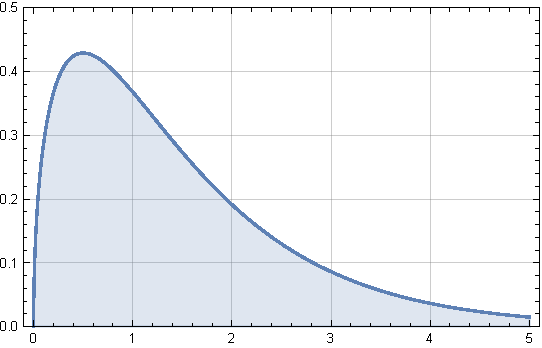
\includegraphics{Mathematica/output/SqrtExp.pdf}
    \end{Figure}
    因此,如果我们将\xrefpeq{7}的积分上限由$x'$改为$\infty$,并不会有太大的误差
    \begin{Equation}&[8]
        I=\Int[0][\infty]x^{1/2}\e^{-x}\dd{x}
    \end{Equation}
    而转化为无穷后,我们就可以将其向高斯积分的方向转化了,令$t=x^{1/2}$,则$\dd{x}=2t\dd{t}$
    \begin{Equation}&[9]
        I=2\Int[0][\infty]t^2\e^{-t^2}\dd{t}
    \end{Equation}
    而高斯积分的结论告诉我们
    \begin{Equation}&[10]
        I=2\frac{\sqrt{\pi}}{4}=\frac{\sqrt{\pi}}{2}
    \end{Equation}
    将\xrefpeq{10}代入\xrefpeq{6}
    \begin{Equation}&[11]
        n_0=\frac{1}{4\pi^{3/2}}\frac{(2\mne)^{3/2}}{\hbar^3}(\kB T)^{3/2}\exp(\frac{E_\text{F}-E_\text{c}}{\kB T})
    \end{Equation}
    我们可以将系数整理为一个统一的$3/2$次项
    \begin{Equation}&[12]
        n_0=\frac{1}{4}\qty(\frac{2\mne\kB T}{\pi\hbar^2})^{3/2}\exp(\frac{E_\text{F}-E_\text{c}}{\kB T})
    \end{Equation}
    我们在系数的括号内除以$4$,这相当于在括号外要乘$4^{3/2}=8$
    \begin{Equation}&[13]
        n_0=2\qty(\frac{\mne\kB T}{2\pi\hbar^2})^{3/2}\exp(\frac{E_\text{F}-E_\text{c}}{\kB T})
    \end{Equation}
    若记\xrefpeq{13}左端的常系数为$N_\text{c}$,我们就可以得到\xrefpeq{A}的结论形式,而依据\fancyref{fml:玻尔兹曼分布},此时\xrefpeq{13}右端的指数项$\exp(E_\text{F}-E_\text{c}/\kB T)$,其实也可以记为$f(E_\text{c})$。
\end{Proof}

\subsection{价带空穴浓度}
\begin{BoxFormula}[价带空穴浓度]
    价带空穴浓度满足
    \begin{Equation}&[A]
        p_0=N_\text{v}\exp(\frac{E_\text{v}-E_\text{F}}{\kB T})=N_\text{v}[1-f(E_\text{v})]
    \end{Equation}
    其中$N_\text{v}$称为价带的有效状态密度,满足
    \begin{Equation}&[B]
        N_\text{v}=2\qty(\frac{\mpe\kB T}{2\pi\hbar^2})^{3/2}
    \end{Equation}
\end{BoxFormula}

\begin{Proof}
    我们仍然从\xrefpeq[载流子浓度]{2}出发,但是这一次$f(E)$需要更换为$1-f(E)$,而$g_\text{c}(E)$需要换为$g_\text{v}(E)$
    \begin{Equation}&[1]
        \dd{n}=\frac{\dd{N}}{V}=\frac{[1-f(E)]g_\text{v}(E)}{V}
    \end{Equation}
    根据\fancyref{fml:价带顶的状态密度}和\fancyref{fml:玻尔兹曼分布}
    \begin{Equation}&[2]
        \dd{n}=\frac{1}{V}\qty[\frac{V}{2\pi^3}\frac{(2\mpe)^{3/2}}{\hbar^3}(E_\text{v}-E)^{1/2}]\qty[\exp(\frac{E-E_\text{F}}{\kB T})]
    \end{Equation}
    将$V$约掉,并对指数部分做一些调整
    \begin{Equation}&[3]
        \dd{n}=\frac{1}{2\pi^2}\frac{(2\mpe)^{3/2}}{\hbar^3}(E_\text{v}-E)^{1/2}\exp(\frac{E_\text{v}-E_\text{F}}{\kB T})\exp(\frac{E-E_\text{v}}{\kB T})
    \end{Equation}
    现在,让我们对$\dd{n}$进行积分
    \begin{Equation}&[4]
        \qquad\qquad
        p_0=\frac{1}{2\pi^2}\frac{(2\mpe)^{3/2}}{\hbar^3}\exp(\frac{E_\text{v}-E_\text{F}}{\kB T})\Int[E_\text{v}'][E_\text{v}]\exp(\frac{E-E_\text{v}}{\kB T})(E_\text{v}-E)^{1/2}\dd{E}
        \qquad\qquad
    \end{Equation}
    后续的步骤是完全相似的,积分后化简为
    \begin{Equation}&[5]
        p_0=2\qty(\frac{\mpe\kB T}{2\pi\hbar^2})^{3/2}\exp(\frac{E_\text{v}-E_\text{F}}{\kB T})
    \end{Equation}
    若记\xrefpeq{5}左端的常系数为$N_\text{v}$,我们就可以得到\xrefpeq{A}的结论形式,而依据\fancyref{fml:玻尔兹曼分布},此时\xrefpeq{5}右端的指数项$\exp(E_\text{v}-E_\text{F}/\kB T)$,其实亦可记为$1-f(E_\text{v})$。
\end{Proof}

\subsection{载流子的浓度乘积}
\begin{BoxFormula}[载流子的浓度乘积]
    载流子的浓度乘积满足
    \begin{Equation}
        n_0p_0=N_\text{c}N_\text{v}\exp(-\frac{E_\text{g}}{\kB T})
    \end{Equation}
    或者展开$N_\text{c},N_\text{v}$
    \begin{Equation}
        n_0p_0=4T^3\qty(\mne\mpe)^{3/2}\qty(\frac{\kB}{2\pi\hbar^2})^3\exp(-\frac{E_\text{g}}{\kB T})
    \end{Equation}
\end{BoxFormula}
\begin{Proof}
    这很容易证明,根据\fancyref{fml:导带电子浓度}和\fancyref{fml:价带空穴浓度}
    \begin{Equation}&[1]
        n_0p_0=N_\text{c}N_\text{v}\exp(\frac{E_\text{F}-E_\text{c}}{\kB T})\exp(\frac{E_\text{v}-E_\text{F}}{\kB T})
    \end{Equation}
    合并两个指数项
    \begin{Equation}&[2]
        n_0p_0=N_\text{c}N_\text{v}\exp(\frac{E_\text{v}-E_\text{c}}{\kB T})
    \end{Equation}
    我们知道禁带宽度$E_\text{g}=E_\text{c}-E_\text{v}$
    \begin{Equation}*
        n_0p_0=N_\text{c}N_\text{v}\exp(-\frac{E_\text{g}}{\kB T})\qedhere
    \end{Equation}
\end{Proof}

\fancyref{fml:载流子的浓度乘积}告诉我们一个重要的事实,\empx{电子和空穴的浓度乘积与费米能级无关}。该结论普遍适用于一切热平衡状态下的非简并半导体,且对本征半导体和杂质半导体都成立。实际上,掺杂改变的主要就是费米能级,故对于某种半导体材料,掺杂与否,掺杂的多少,并不会改变$n_0p_0$的结果,这会为我们之后讨论杂质半导体带来很多便利,比如
\begin{itemize}
    \item 如果掺杂使得电子浓度增加,那么空穴浓度必然会减少。
    \item 如果掺杂使得空穴浓度增加,那么空穴浓度必然会减少。
\end{itemize}
该结论还指出$n_0p_0$大致正比于$T^3$(在$T$较大时$\exp(-E_\text{g}/\kB T)$将趋向于$1$),这就表明,载流子的浓度乘积会随着温度增加而迅速增加,换言之,温度对于半导体的导电性的影响很大。
\section{本征半导体的载流子浓度}
\uwave{本征半导体}(Intrinsic Semiconductor)就是指一块没有杂质和缺陷的半导体,因此,本征半导体的载流子完全来自本征激发,由于本征激发中,电子从价带跃迁到导带,电子和空穴将会成对产生,因此,导带中的电子浓度应当等同于价带中的空穴浓度,这就是\uwave{电中性条件}。

\begin{BoxFormula}[本征半导体的电中性条件]
    本征半导体的电中性条件满足
    \begin{Equation}
        n_0=p_0
    \end{Equation}
\end{BoxFormula}

本征半导体的能带图,如\xref{fig:本征半导体的能带图}所示,其中,需要特别解释的是最右侧的图像,我们可能会困惑其中的$\dv*{n_0}{E}$和$\dv*{p_0}{E}$究竟是什么含义?介于$n_0$和$p_0$本身就是对能量$E$积分后的常数,又何谈对$E$的导数呢?实际上,在\xref{sec:载流子浓度}当我们通过积分求得$n_0$和$p_0$时,被积函数就是$f(E)g(E)/V$,它表征了载流子浓度的能量密度。原先的观点中$n_0,p_0$由能带底到能带顶的定积分,如果放宽一些,将$n_0,p_0$视为由能带顶到$E$的变上限积分$n_0(E),p_0(E)$,那这里的$\dv*{n_0}{E}$和$\dv*{p_0}{E}$就可以解释了,它们与$f(E)g(E)/V$是同一回事,都代表浓度的能量密度。这也是为何$f(E)g(E)/V$的曲线下面积就表示了电子浓度$n_0$和空穴浓度$p_0$的大小。
\begin{Figure}[本征半导体的能带图]
    \includegraphics[width=0.95\linewidth]{build/Chapter03D_03.fig.pdf}
\end{Figure}

这里也证实了先前的一个提法,我们注意到
\begin{itemize}
    \item 导带电子浓度的能量密度的最大值接近导带底,表明,\empx{导带电子主要位于导带底}。
    \item 价带电子浓度的能量密度的最大值接近价带顶,表明,\empx{价带空穴主要位于价带顶}。
\end{itemize}
这里关注到\xref{fig:本征半导体的能带图}中$f(E)$和$g(E)$的图像相较\xref{fig:状态密度函数}和\xref{fig:费米分布与玻尔兹曼分布},作为自变量的能量反而变为了纵轴,这其实是为了顺应简单能带图中,能量在纵向分布的习惯,也是半导体物理的通用作法。


至此,有一个疑惑,这一节我们到底要干嘛?本节题名“本征半导体的载流子浓度”,但问题是,载流子的浓度我们在\xref{sec:载流子浓度}中,已经由\fancyref{fml:导带电子浓度}和\fancyref{fml:价带空穴浓度}求出了,本节还有什么可做的?关键点在于,现有的$n_0$和$p_0$的公式中包含费米能级$E_\text{F}$,而根据固体物理的知识,\empx{费米能级是随温度变化的函数},而这个函数是我们目前未知的。因此,本节就是要求出本征半导体的费米能级的函数,进而求出$n_0$和$p_0$的具体表达。

\begin{BoxFormula}[本征半导体的费米能级]*
    本征半导体的费米能级满足
    \begin{Equation}
        E_\text{F}=\frac{E_\text{c}-E_\text{v}}{2}+\frac{\kB T}{2}\ln\frac{N_\text{v}}{N_\text{c}}
    \end{Equation}
    或
    \begin{Equation}
        E_\text{F}=E_\text{i}=\frac{E_\text{c}+E_\text{v}}{2}+\frac{3\kB T}{4}\ln\frac{\mpe}{\mne}
    \end{Equation}
    这里$E_\text{i}$是专属本征半导体的费米能级的记号,下标i表示本征(Intrinsic)。
\end{BoxFormula}
\begin{Proof}
    求解费米能级的关键,在于运用电中性条件,根据\fancyref{fml:本征半导体的电中性条件}
    \begin{Equation}&[1]
        n_0=p_0
    \end{Equation}
    根据\fancyref{fml:导带电子浓度}和\fancyref{fml:价带空穴浓度}
    \begin{Equation}&[2]
        N_\text{c}\exp(\frac{E_\text{F}-E_\text{c}}{\kB T})=N_\text{v}\exp(\frac{E_\text{v}-E_\text{F}}{\kB T})
    \end{Equation}
    在\xrefpeq{2}两端取对数
    \begin{Equation}&[3]
        \ln N_\text{c}+\qty(\frac{E_\text{F}-E_\text{c}}{\kB T})=\ln N_\text{V}+\qty(\frac{E_\text{v}}{\kB T})
    \end{Equation}
    移项整理
    \begin{Equation}&[4]
        \frac{2E_\text{F}-E_\text{c}-E_\text{v}}{\kB T}=\ln\frac{N_\text{v}}{N_\text{c}}
    \end{Equation}
    再整理
    \begin{Equation}&[5]
        \frac{2E_\text{F}}{\kB T}=\frac{E_\text{c}-E_\text{v}}{\kB T}+\ln\frac{N_\text{v}}{N_\text{c}}
    \end{Equation}
    由此即解得$E_\text{F}$
    \begin{Equation}&[6]
        E_\text{F}=\frac{E_\text{c}-E_\text{v}}{2}+\frac{\kB T}{2}\ln\frac{N_\text{v}}{N_\text{c}}
    \end{Equation}
    而我们知道$N_\text{v}\sim(\mpe)^{3/2}$和$N_\text{c}\sim(\mne)^{3/2}$
    \begin{Equation}&[7]
        E_\text{F}=\frac{E_\text{c}-E_\text{v}}{2}+\frac{3\kB T}{4}\ln\frac{\mpe}{\mne}
    \end{Equation}
    这里,我们愿意引入$E_\text{i}$作为本征半导体中费米能级$E_\text{F}$的特别记号。
\end{Proof}

\xref{fml:本征半导体的费米能级}指出,本征半导体的费米能级$E_\text{i}$由两部分组成,首先是$E_\text{c}+E_\text{v}/2$的常数部分,它表明费米能级在绝对零度时位于禁带中线上,其次是$(3\kB T/4)\ln(\mpe/\mne)$的线性项,它表明费米能级将随温度增大线性变化。不过事实上,对于大部分半导体材料,在室温范围内,线性项的影响其实都不大。例如,根据\xref{tab:半导体的状态密度有效质量}的数据,硅和锗的$\mpe/\mne$分别为$0.55$和$0.52$,砷化镓的$\mpe/\mne$则为$8.25$,故三者的$\ln(\mpe/\mne)$均大致在$\pm 2$的范围内,而$\kB T$在室温$T=300\si{K}$时为$\kB T=0.026\si{eV}$,因此整个线性项在室温下的影响小于$0.05\si{eV}$,根据\xref{tab:部分半导体材料的参数}的数据,其相较于硅、锗、砷化镓$1.14\si{eV}, 0.67\si{eV}, 1.52\si{eV}$在$1\si{eV}$量级的禁带宽度,完全可以忽略,因此我们可以近似认为,\empx{本征半导体的费米能级基本在禁带中线附近}。不过,也有例外,例如锑化铟的$\mpe/\mne$约为$36.7$,取对数后仍然有$3.60$,线性项的影响达到了近$0.07\si{eV}$,但是,锑化铟的禁带非常窄,仅有$0.17\si{eV}$,这时,线性项的影响就很显著了,费米能级已远在禁带中线上了。

现在,让我们来计算本征半导体的载流子浓度。

\begin{BoxFormula}[本征半导体的载流子浓度]
    本征半导体中,电子浓度$n_0$和空穴浓度$p_0$相等,统一记为$n_\text{i}$
    \begin{Equation}
        n_\text{i}=n_0=p_0
    \end{Equation}
    且$n_\text{i}$满足
    \begin{Equation}
        n_\text{i}=(N_\text{c}N_\text{v})^{1/2}\exp(-\frac{E_\text{g}}{2\kB T})
    \end{Equation}
\end{BoxFormula}

\begin{Proof}
    根据\fancyref{fml:导带电子浓度},并代入\fancyref{fml:本征半导体的费米能级}
    \begin{Equation}&[1]
        \qquad
        n_0=N_\text{c}\exp(\frac{E_\text{F}-E_\text{c}}{\kB T})=N_\text{c}\exp(\frac{E_\text{c}/2+E_\text{v}/2+(\kB T/2)\ln N_\text{v}/N_\text{c}-E_\text{c}}{\kB T})
        \qquad
    \end{Equation}
    化简整理得
    \begin{Equation}&[2]
        n_0=N_\text{c}\qty(-\frac{E_\text{c}-E_\text{v}}{2\kB T}+\frac{\ln N_\text{v}/N_\text{c}}{2})=N_\text{c}\sqrt{N_\text{v}/N_\text{c}}\exp(-\frac{E_\text{g}}{2\kB T})=(N_\text{c}N_\text{v})^{1/2}\exp(-\frac{E_\text{g}}{2\kB T})
    \end{Equation}
    根据\fancyref{fml:价带空穴浓度},并代入\fancyref{fml:本征半导体的费米能级}
    \begin{Equation}&[3]
        \qquad
        p_0=N_\text{v}\exp(\frac{E_\text{v}-E_\text{F}}{\kB T})=N_\text{c}\exp(\frac{E_\text{v}-E_\text{c}/2-E_\text{v}/2-(\kB T/2)\ln N_\text{v}/N_\text{c}}{\kB T})
        \qquad
    \end{Equation}
    化简整理得
    \begin{Equation}&[4]
        p_0=N_\text{v}\qty(-\frac{E_\text{c}-E_\text{v}}{2\kB T}-\frac{\ln N_\text{v}/N_\text{c}}{2})=N_\text{v}\sqrt{N_\text{c}/N_\text{v}}\exp(-\frac{E_\text{g}}{2\kB T})=(N_\text{v}N_\text{c})^{1/2}\exp(-\frac{E_\text{g}}{2\kB T})
    \end{Equation}
    比较\xrefpeq{3}和\xrefpeq{4}即得
    \begin{Equation}*
        n_0=p_0\qedhere
    \end{Equation}
\end{Proof}
由此可见,本征半导体的载流子浓度对温度非常敏感,其随温度增加而迅速增加。而在同一温度下,半导体材料的禁带宽度$E_\text{g}$越大,本征载流子的浓度$n_i$就相应越小,这从直观上想也是很合理的,因为禁带宽度越大,电子从价带跃迁到导带也越困难,载流子自然也就少了。

在\xref{fml:本征半导体的载流子浓度}中代入$N_\text{c}N_\text{v}$,并引入\fancyref{fml:禁带宽度和温度的关系}
\begin{Equation}
    n_i=2\frac{(2\pi \kB T)^{3/2}(\mpe\mne)^{3/4}}{\hbar^3}\exp[-\frac{E_\text{g}(0)}{2\kB T}]\exp[\frac{\alpha T}{2\kB (T+\beta)}]
\end{Equation}
该式可以在实验上用于测定禁带宽度。